\documentclass[11pt]{article}

\usepackage[margin=0.85in]{geometry}
\usepackage[T1]{fontenc}
\usepackage[utf8]{inputenc}
\usepackage{lmodern}
\usepackage{microtype}
\usepackage{graphicx}
\usepackage{booktabs}
\usepackage{amsmath}
\usepackage{hyperref}
\usepackage{caption}
\usepackage{float}

\hypersetup{
  colorlinks=true,
  linkcolor=blue,
  citecolor=blue,
  urlcolor=blue
}

\newcommand{\outputroot}{/home/lachlan/ProjectsLFS/OrganoidAgent/analysis-outputs/yichao_future_expression}

\title{\textbf{Yichao Joint Training Results: B2F-Assisted Future Fluorescence Prediction}}
\author{OrganoidAgent Yichao analysis}
\date{May 11, 2026}

\begin{document}
\maketitle

\begin{abstract}
This report covers only the joint Yichao model trained in stage 3. The joint model used current brightfield history to predict future fluorescence while also reconstructing current fluorescence as an auxiliary B2F task. The held-out test set contains 633 future samples and 11 future-expression examples. The model achieved future image MAE 0.3112, future image PSNR 7.95 dB, current auxiliary B2F image MAE 0.2173, expression AUROC 0.223, future peak Pearson correlation -0.049, and future AUC Pearson correlation 0.075. The joint idea remains the better modeling direction than a scalar-only separate model, but the current implementation does not yet predict future fluorescence close to truth.
\end{abstract}

\section{Scope}

This document intentionally excludes the separately trained B2F and scalar future reports. It uses only the stage3 joint output:

\begin{center}
\small
\path{\outputroot/stage3_joint_b2f_future}
\end{center}

The model was trained with image size 256, maximum prefix length 5, last-future target policy, batch size 16, learning rate $2\times10^{-4}$, mixed precision, and CUDA.

\section{Joint Model}

The joint model receives a brightfield prefix and explicit morphology/time features:
\begin{equation}
P_k = \{(B_j, X_j)\}_{j=k-L+1}^{k}, \quad L \leq 5.
\end{equation}

It predicts four groups of outputs:
\begin{equation}
(\hat{F}_{p}, \hat{F}_{k}, \hat{y}_{p}, \hat{s}_{p})
= J_\psi(P_k), \quad p > k,
\end{equation}
where $\hat{F}_{p}$ is future fluorescence, $\hat{F}_{k}$ is current auxiliary fluorescence reconstruction, $\hat{y}_{p}$ is future-expression probability, and $\hat{s}_{p}$ contains scalar future intensity targets.

The training objective combines dense future image loss, current B2F auxiliary loss, and scalar future losses:
\begin{equation}
\mathcal{L}
= \mathcal{L}_{\mathrm{future\ image}}
+0.5\mathcal{L}_{\mathrm{current\ B2F}}
+0.25\mathcal{L}_{\mathrm{future\ scalar}}
+0.05\mathcal{L}_{\mathrm{current\ scalar}}.
\end{equation}

\section{Held-Out Metrics}

\begin{table}[H]
\centering
\caption{Stage3 joint held-out test metrics from \texttt{stage3\_joint\_b2f\_future/test\_metrics.json}.}
\begin{tabular}{lc}
\toprule
Metric & Value \\
\midrule
Test future samples & 633 \\
Future-expression examples & 11 \\
Future image MAE & 0.3112 \\
Future image MSE & 0.1603 \\
Future image PSNR & 7.95 dB \\
Current auxiliary B2F image MAE & 0.2173 \\
Expression AUROC & 0.223 \\
Average precision & 0.0127 \\
Future peak Pearson correlation & -0.049 \\
Future AUC Pearson correlation & 0.075 \\
Future peak MAE & 0.603 \\
Future AUC MAE & 0.955 \\
Best epoch & 2 \\
\bottomrule
\end{tabular}
\end{table}

\begin{figure}[H]
\centering
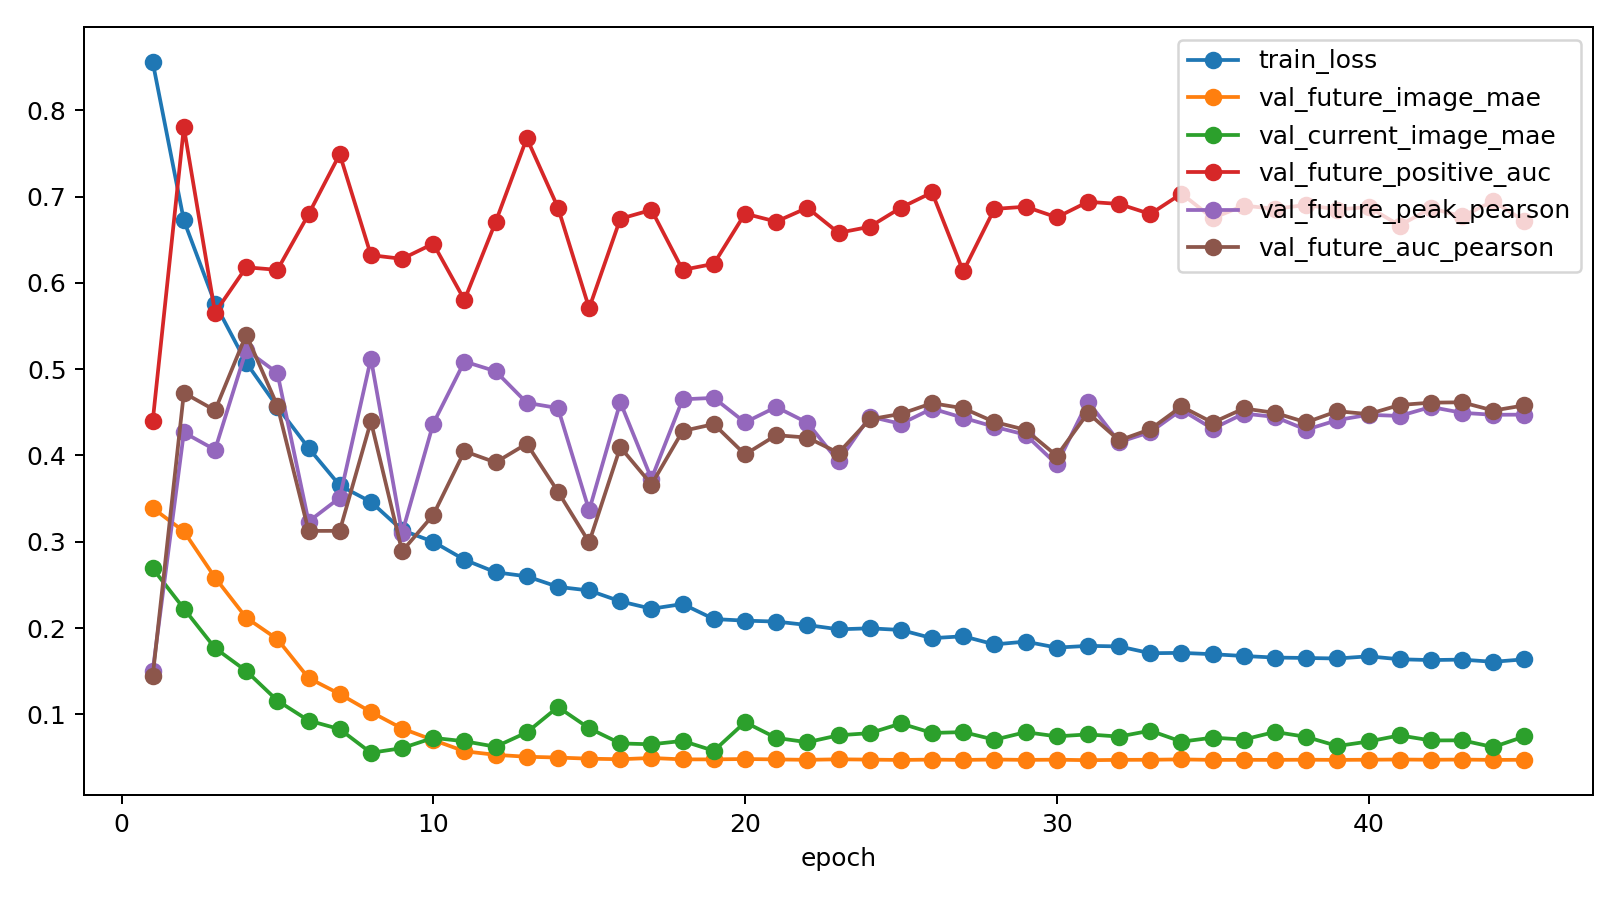
\includegraphics[width=0.92\linewidth]{figures/fig1_joint_training_metrics.png}
\caption{Joint model training curves from the stage3 run.}
\label{fig:joint-training}
\end{figure}

\begin{figure}[H]
\centering
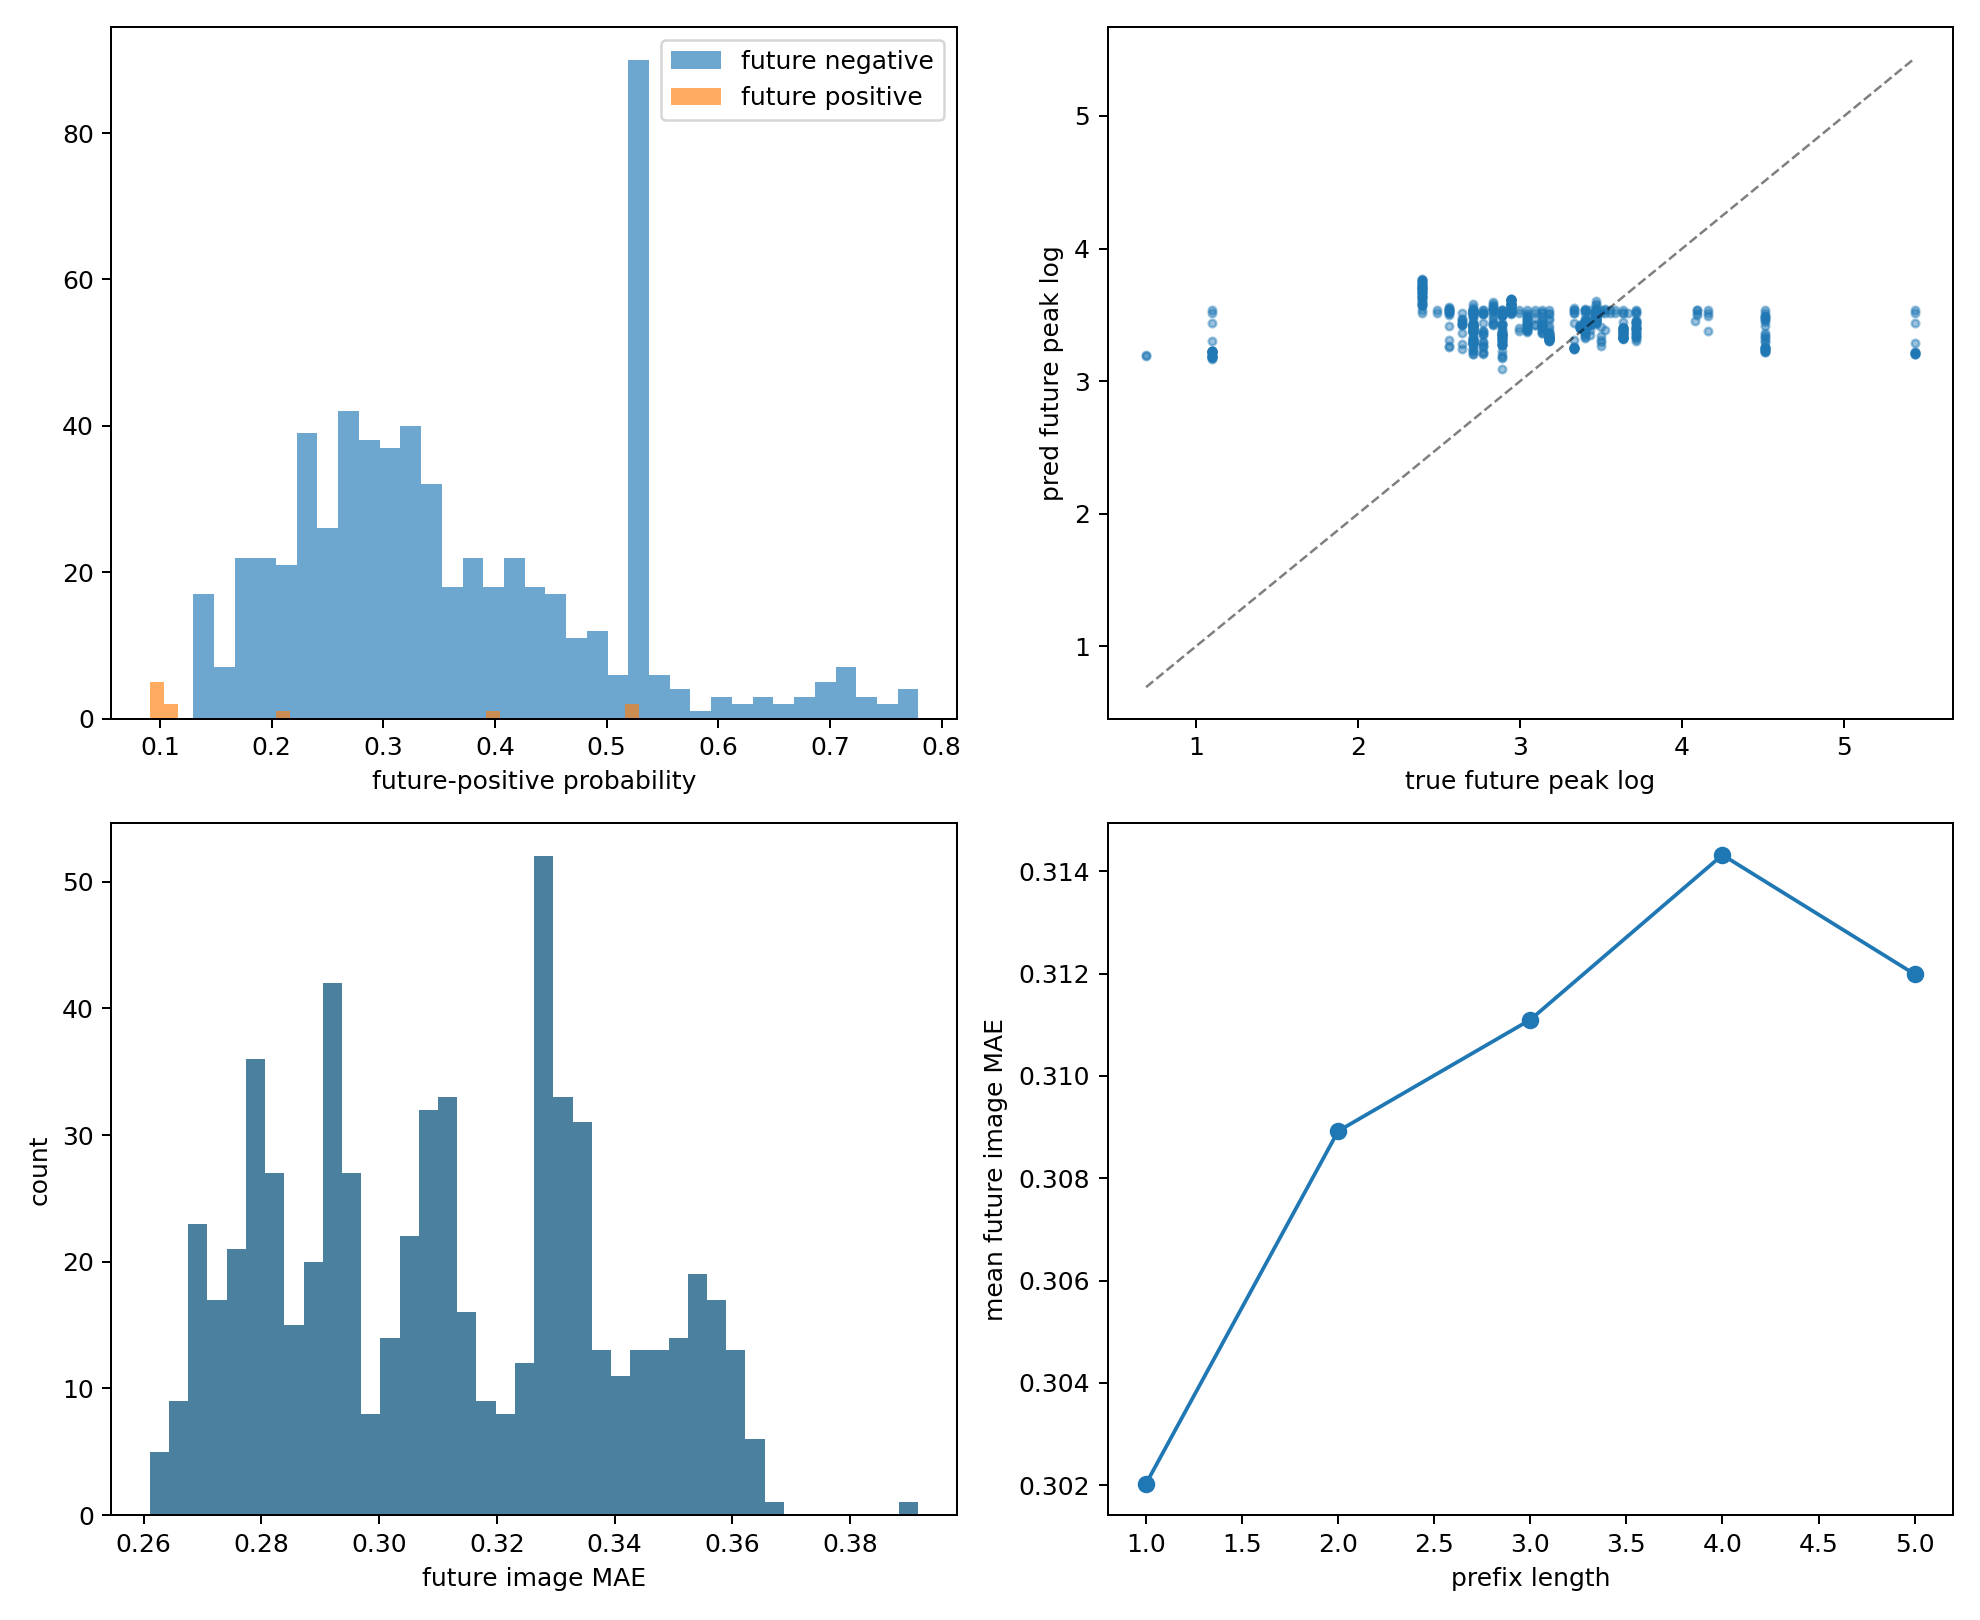
\includegraphics[width=\linewidth]{figures/fig2_joint_summary.png}
\caption{Joint model held-out summary.}
\label{fig:joint-summary}
\end{figure}

\begin{figure}[H]
\centering
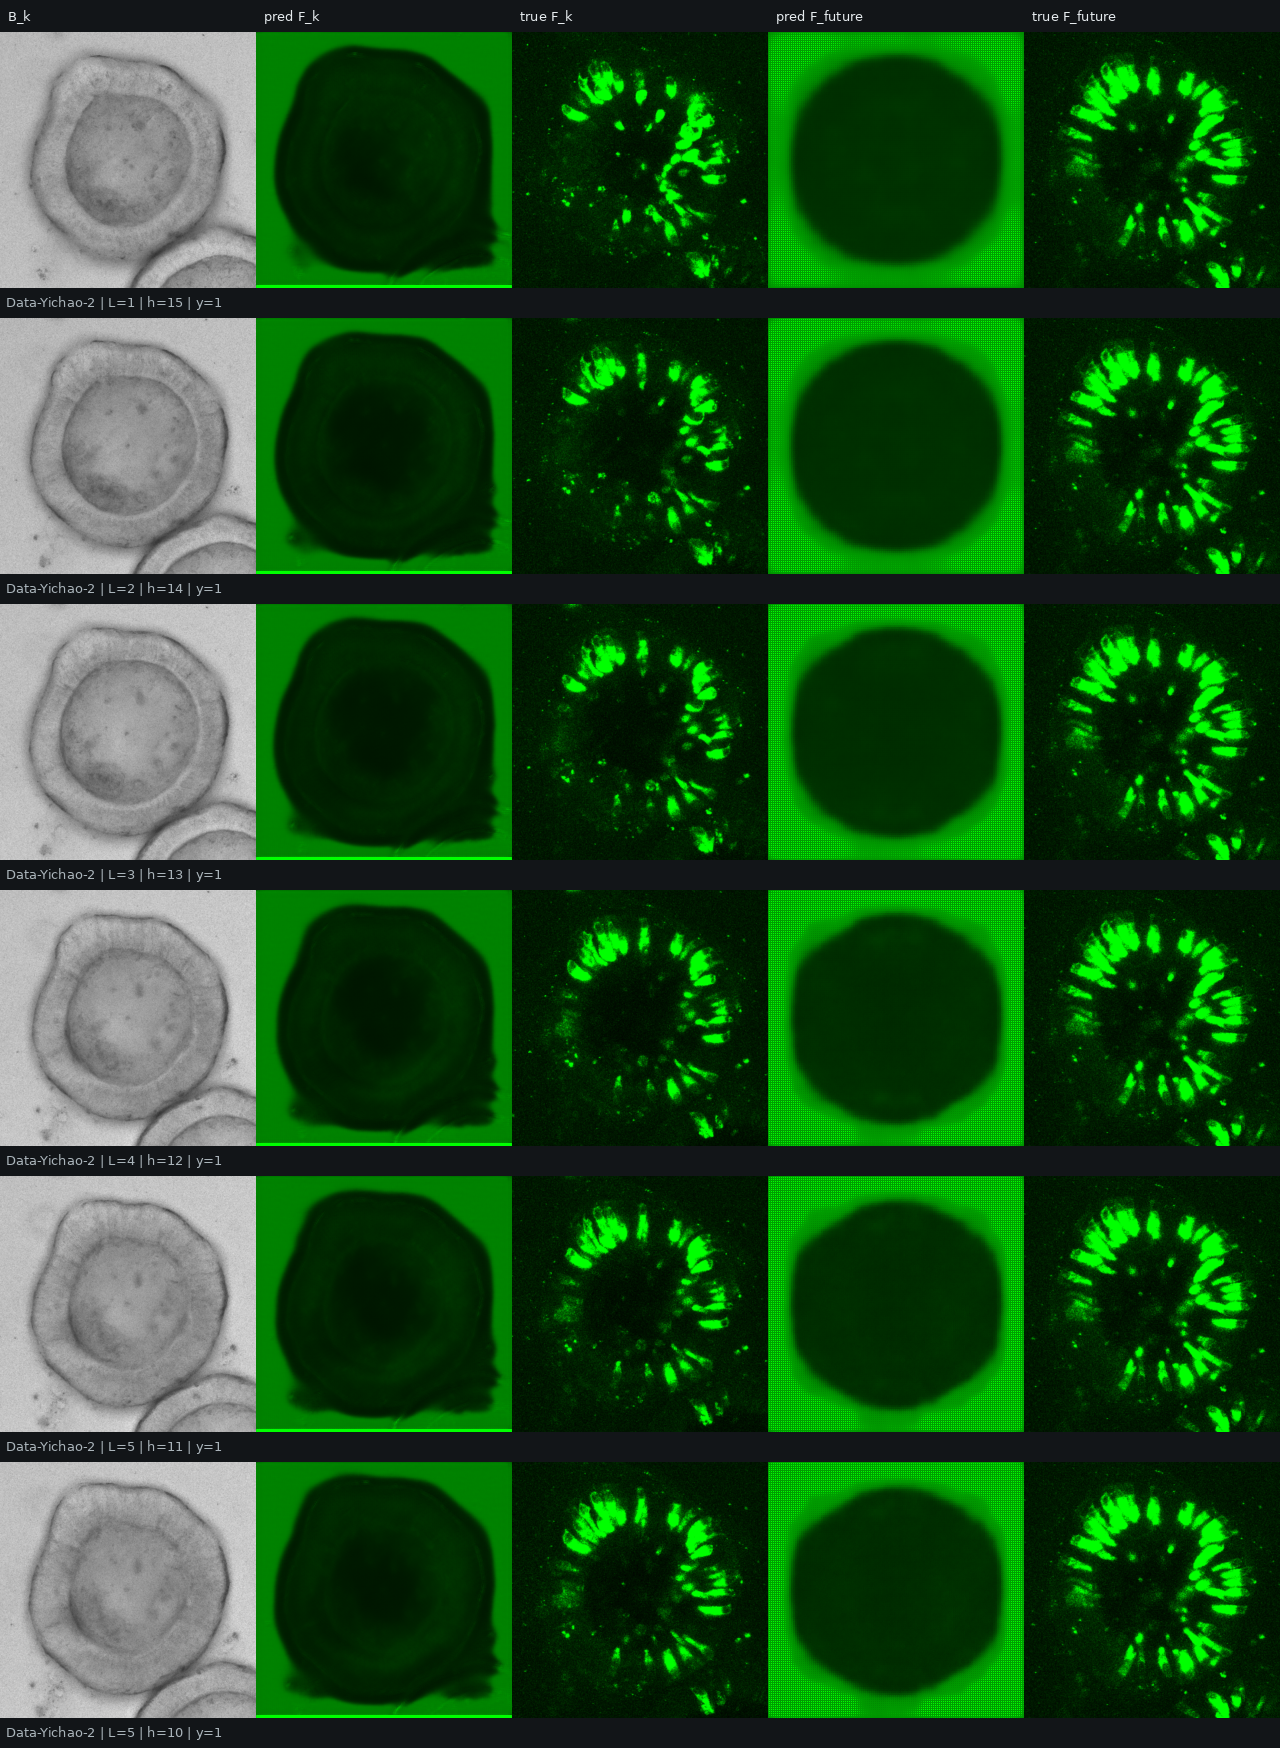
\includegraphics[height=0.82\textheight,keepaspectratio]{figures/fig3_joint_test_predictions.png}
\caption{Joint held-out prediction panel. Columns show current brightfield, predicted current fluorescence, true current fluorescence, predicted future fluorescence, and true future fluorescence. The visual mismatch shows that the future image prediction is not yet close to the target.}
\label{fig:joint-predictions}
\end{figure}

\section{Feature Ablation}

\begin{figure}[H]
\centering
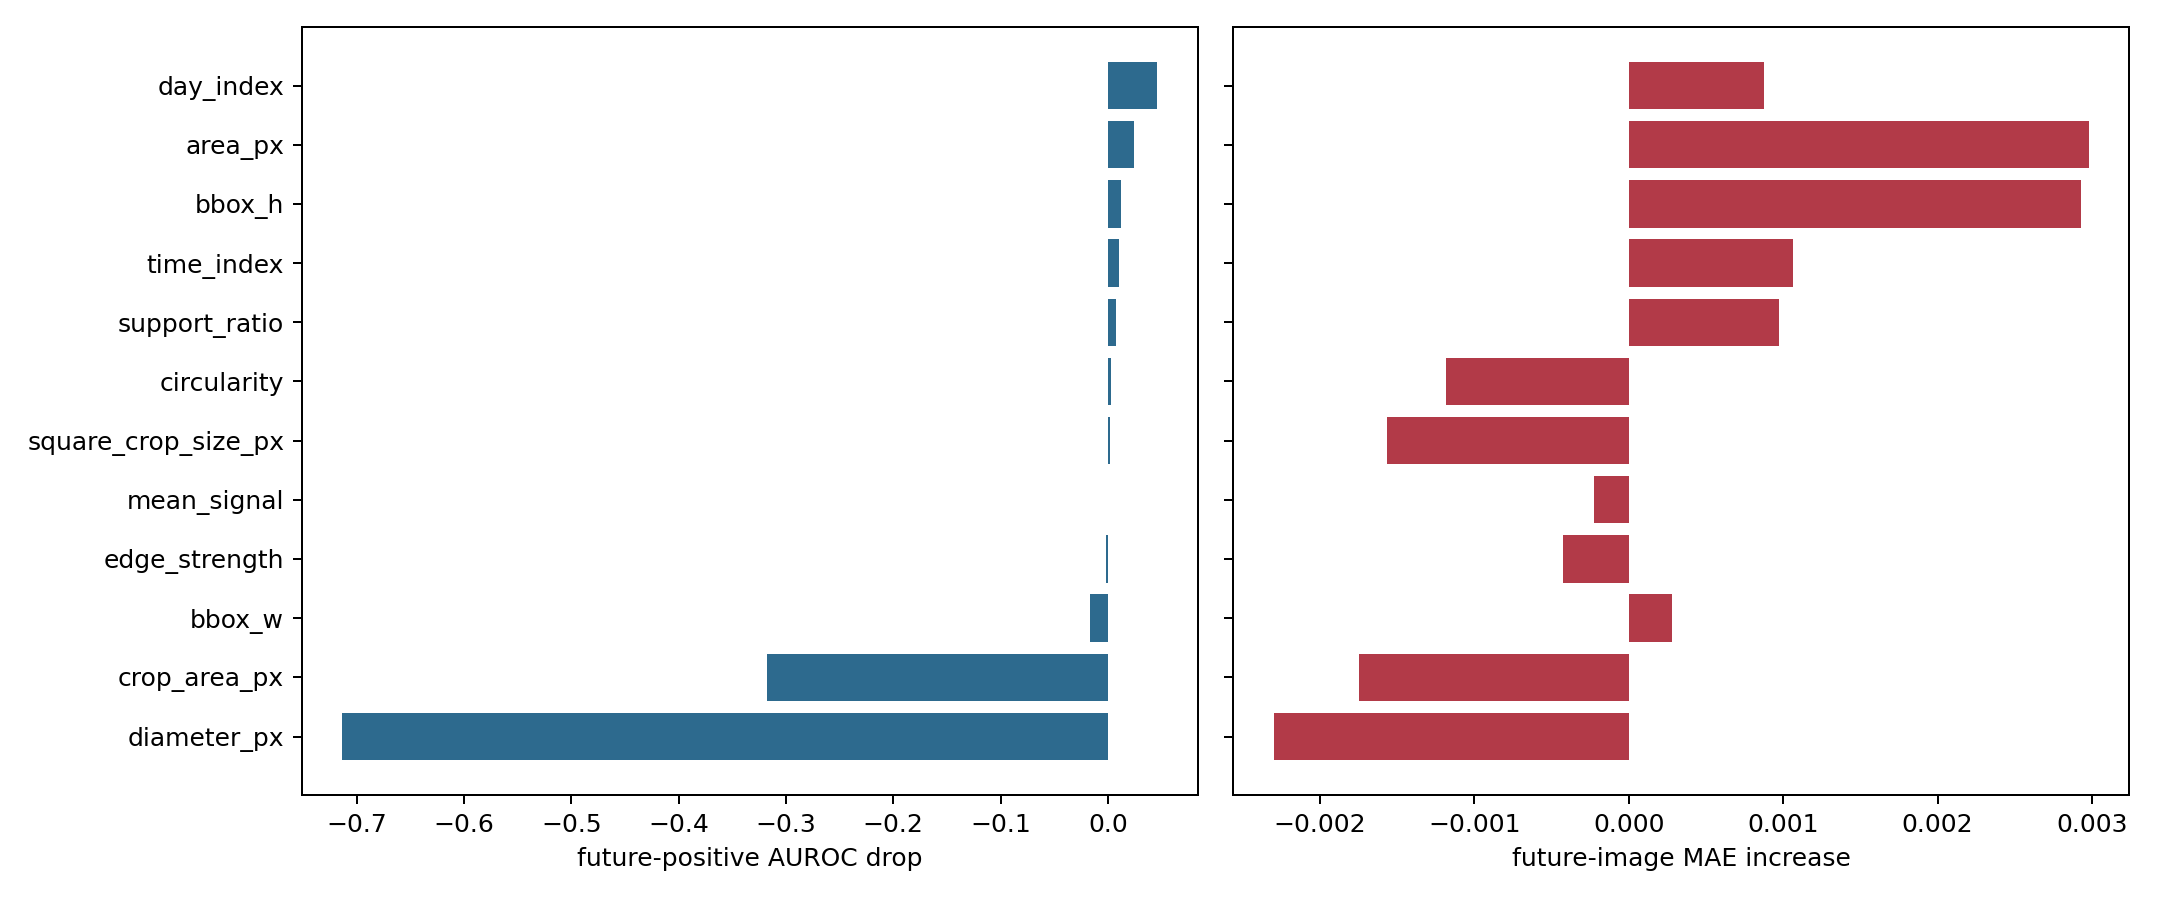
\includegraphics[width=0.92\linewidth]{figures/fig4_joint_feature_ablation.png}
\caption{Stage3 feature ablation summary.}
\label{fig:joint-ablation}
\end{figure}

\begin{table}[H]
\centering
\caption{Top stage3 feature ablations from \texttt{joint\_b2f\_future\_report.md}.}
\begin{tabular}{lccc}
\toprule
Feature & AUROC drop & Future image MAE increase & Peak-correlation drop \\
\midrule
Day index & 0.046 & 0.0009 & 0.109 \\
Area & 0.024 & 0.0030 & -0.112 \\
Bounding-box height & 0.013 & 0.0029 & 0.059 \\
Time index & 0.011 & 0.0011 & -0.043 \\
Support ratio & 0.007 & 0.0010 & -0.037 \\
Circularity & 0.003 & -0.0012 & -0.002 \\
Square crop size & 0.002 & -0.0016 & 0.032 \\
Mean signal & 0.001 & -0.0002 & 0.023 \\
\bottomrule
\end{tabular}
\end{table}

\section{Interpretation}

The joint result answers a different question from separate training. It tests whether current B2F reconstruction can regularize a future-fluorescence predictor. The answer from this run is: the concept is still the better direction, but the implementation and target design are not yet strong enough.

Three observations matter:

\begin{enumerate}
\item The future image output is visibly not close to the true future fluorescence.
\item The future-expression ranking metric is weak on the held-out split.
\item The auxiliary current B2F head is worse than the separately trained B2F model, suggesting that the joint network capacity and loss balance are not yet adequate.
\end{enumerate}

\section{How To Improve The Joint Model}

The next joint model should be bolder, but not blindly larger. The priority order should be:

\begin{enumerate}
\item \textbf{Initialize from the separate B2F encoder.} The separate B2F task already learned useful morphology-to-fluorescence features. The joint model should start from those weights instead of relearning them.
\item \textbf{Increase resolution.} Keep 256$\times$256 for fast debugging, but train the serious model at 384$\times$384 or 512$\times$512. Yichao's described signal is thin peripheral fluorescent cell morphology with possible internal voids, and 256 can lose this structure.
\item \textbf{Increase capacity moderately.} The current joint model used base channels 16. A stronger run should use a ResNet/ConvNeXt-style encoder or U-Net encoder with 32--64 base channels, mixed precision, and gradient accumulation.
\item \textbf{Use temporal attention or a GRU over frame embeddings.} A simple prefix average is too weak for $D_1,\ldots,D_k \rightarrow D_p$. The model should learn which day/frame is informative.
\item \textbf{Train horizon-specific heads.} Predict $D_{k+1}$, $D_{k+2}$, and peak-future separately instead of collapsing all futures into one last-future target.
\item \textbf{Balance expression trajectories.} Oversample future-expression tracks and add a ranking loss so the model learns relative risk of future expression.
\item \textbf{Audit temporal tracks.} Wrong linked organoids directly corrupt the future target. This likely matters more than adding parameters.
\end{enumerate}

The recommended next architecture is:
\begin{equation}
e_j = E_{\theta}(B_j), \quad
z_k = T_{\phi}\left((e_1,X_1), \ldots, (e_k,X_k)\right),
\end{equation}
\begin{equation}
(\hat{F}_k,\hat{F}_{k+1},\hat{F}_{k+2},\hat{F}_{\mathrm{peak}},\hat{y}_{\mathrm{future}},\hat{s}_{\mathrm{future}})
= D_{\psi}(z_k),
\end{equation}
where $E_\theta$ is initialized from the separate B2F model, $T_\phi$ is a temporal encoder, and $D_\psi$ contains current, short-horizon, and peak-future heads.

\section{Conclusion}

The joint model is the more realistic direction for the biological goal, but this specific stage3 run does not yet predict future fluorescence well. The next run should use B2F-pretrained initialization, larger image size, more capacity, horizon-specific targets, and audited tracks. The goal is not only to improve image similarity, but to identify the earliest day $k$ where $B_{1:k}$ contains enough information to predict later fluorescence expression.

\end{document}
